%\documentclass[wcp,gray]{jmlr}
\documentclass[wcp]{jmlr}

\usepackage{booktabs}
\usepackage{longtable}
\usepackage{graphicx}
\usepackage{amsmath,amssymb}
\usepackage{hyperref}
\usepackage{lineno}
% \linenumbers

\pagenumbering{gobble}
\newcommand{\cs}[1]{\texttt{\char`\\#1}}
\makeatletter
\let\Ginclude@graphics\@org@Ginclude@graphics
\makeatother

\jmlryear{2026}
\jmlrworkshop{ACML 2026}

\title[Bayesian Fusion for Multi-Sensor Damage Assessment]{Bayesian Uncertainty Fusion for Multi-Sensor Remote Sensing Damage Assessment:\\A Case Study of Sentinel-2 and VIIRS in Mariupol}

\author{
  \Name{Author Name} \Email{author@university.edu}\\
  \addr{Department of Statistics, University Name}
}

\editors{}

\begin{document}

\makeatletter
\let \@jmlrpages \@empty
\makeatother

\maketitle

%=====================================================================
\begin{abstract}
Multi-sensor fusion is widely used in remote sensing damage assessment,
yet the consequences of combining sensors that measure distinct damage
dimensions remain underexplored. This study fuses Sentinel-2 (S2) spectral
indices and VIIRS nighttime light (NTL) loss to estimate war-related damage
in Mariupol, Ukraine, under a Bayesian hierarchical uncertainty framework.
We find that S2 and VIIRS each contain meaningful spatial information, but
their signals systematically disagree---S2 primarily captures surface
alteration, while VIIRS registers functional cessation through reduced
nighttime illumination. When forced into a single latent damage state, the
Bayesian posterior collapses to a near-uniform spatial estimate
($p \approx 0.155$), losing essentially all grid-level differentiation
(KL divergence vs.\ global mean $\approx 0$). Kullback-Leibler and
Jensen-Shannon divergence analysis quantifies a fusion suppression ratio of
$46.8\%$, demonstrating that nearly half of the best single-sensor
information is suppressed under the joint model. Dempster-Shafer evidence
theory preserves uncertainty through belief/plausibility intervals
(Belief~$=0.145$, Plausibility~$=0.369$) but may over-weight strong
single-sensor evidence in the absence of hierarchical shrinkage.
Grid-level consistency comparison reveals approximately $50\%$ genuine
agreement, $10\%$ uncertainty-driven compatibility, and $28\%$ divergence
between the two fusion paradigms. We conclude that adding sensors does not
automatically improve damage estimation accuracy; multi-sensor fusion is
beneficial only when sensors measure compatible damage dimensions or when
the model explicitly accommodates multiple latent states.
\end{abstract}

\begin{keywords}
Bayesian hierarchical model; Dempster-Shafer evidence theory;
Kullback-Leibler divergence; multi-sensor fusion; damage assessment;
Sentinel-2; VIIRS
\end{keywords}

%=====================================================================
\section{Introduction}\label{sec:intro}

Rapid damage assessment following natural disasters and armed conflicts is
critical for humanitarian response and reconstruction planning. Satellite
remote sensing offers a scalable, repeatable means of surveying affected
areas where ground access is limited or unsafe. Optical sensors such as
Sentinel-2 (S2) detect surface changes through pre- and post-event spectral
comparison, while low-light imagers such as the Visible Infrared Imaging
Radiometer Suite (VIIRS) Day-Night Band (DNB) capture reductions in
nighttime illumination associated with infrastructure destruction,
power outages, and population displacement \cite{roman2018,zhang2023}.

A fundamental challenge arises when multiple sensors are combined to produce
a unified damage estimate. Different sensors measure different physical
quantities: S2 spectral indices respond to exposed rubble, soil, and altered
vegetation---manifestations of structural damage---while VIIRS nighttime
light (NTL) loss registers reduced human activity, including power failures
and evacuation. These are not redundant observations of a single latent
damage state; they are complementary but potentially conflicting signals
\cite{xiao2024}. When such conflicting evidence is fused under the
assumption of a single latent damage state, the estimated posterior may
exhibit counterintuitive behavior, including severe shrinkage toward the
population mean and loss of spatial differentiation.

This study addresses three questions: (1)~How do S2 and VIIRS each align
with an external reference under this validation setting? (2)~How does a
Bayesian hierarchical model reconcile conflicting multi-sensor evidence?
(3)~Does adding a second sensor improve estimation accuracy?
We investigate these questions through a case study of Mariupol, Ukraine,
which experienced extensive damage during the 2022 Russia-Ukraine conflict.
We construct S2 spectral damage indices and VIIRS NTL loss indicators at a
500~m grid resolution, validate against UNOSAT reference labels, and apply
three complementary analytical frameworks: Bayesian hierarchical modeling,
KLD/JSD information gain analysis, and Dempster-Shafer (D-S) evidence
theory. The principal contributions of this work are:

\begin{enumerate}
  \item A Bayesian hierarchical uncertainty framework for fusing S2 and
    VIIRS damage probabilities without requiring ground-truth labels.
  \item A quantitative decomposition of single-sensor information, fused
    information, and inter-sensor conflict using KLD and JSD.
  \item A grid-level comparison of Bayesian point-estimate fusion with D-S
    interval-based evidence combination, revealing how the two paradigms
    diverge under conflicting evidence.
\end{enumerate}

%=====================================================================
\section{Study Area and Data}\label{sec:data}

\subsection{Mariupol Area of Interest}

The study area covers the city of Mariupol and its surroundings in
southeastern Ukraine (37.42\textdegree{}E--37.72\textdegree{}E,
47.05\textdegree{}N--47.18\textdegree{}N). Mariupol was a major
battleground during the 2022 Russia-Ukraine conflict, suffering extensive
structural damage to residential, industrial, and infrastructure assets.
The area of interest (AOI) spans approximately 23~km (east-west) by 14~km
(north-south) and is divided into 1{,}380 grid cells at 500~m spatial
resolution.

\subsection{Sentinel-2 Imagery}

We use Sentinel-2 Level-2A surface reflectance products for pre-event
(2021-05-23) and post-event (2022-05-08) acquisitions, covering tiles
T37TCN and T37TDN. The pre-event date was selected to match the same
phenological period one year prior to minimize seasonal vegetation effects.
Spectral indices including the Normalized Difference Vegetation Index
(NDVI), Normalized Burn Ratio (NBR), and soil-adjusted indices were
computed from the 10~m and 20~m bands and aggregated to 500~m grid cells.

\subsection{VIIRS Nighttime Light Data}

VIIRS DNB monthly composite data (VNP46A3) were obtained for the matching
pre- and post-event periods. The DNB radiance values were filtered using the
mandatory quality flag to exclude cloud-contaminated and poor-quality
retrievals. Per-grid mean NTL radiance and the NTL loss rate (relative
reduction from pre- to post-event) were computed at 500~m resolution.

\subsection{UNOSAT External Reference Labels}

UNOSAT damage assessment data for the Livoberezhnyi District of Mariupol,
produced through visual interpretation of very-high-resolution satellite
imagery (dated 12 May 2022), were used as an external reference. Building
footprints with damage classifications were spatially joined to the 500~m
grid. A strict matching protocol was applied, requiring direct spatial
overlap. The resulting validation set contains 995 labeled grids (32.8\%
positive for visible building damage). We emphasize that UNOSAT is used as
an external reference rather than absolute ground truth; it captures
visually identifiable structural damage but may miss functional damage or
sub-detection-threshold structural alteration.

\begin{table}[htp]
\centering
\caption{Data sources and preprocessing summary.}
\label{tab:data}
\begin{tabular}{@{}lllll@{}}
\toprule
\textbf{Data Source} & \textbf{Product} & \textbf{Pre-Date} & \textbf{Post-Date} & \textbf{Resolution} \\
\midrule
Sentinel-2 MSI  & L2A Surface Reflectance & 2021-05-23 & 2022-05-08 & 10--20~m (500~m grid) \\
VIIRS DNB       & VNP46A3 Monthly Composite & 2021-05 & 2022-05 & 500~m native \\
UNOSAT          & Damage Assessment (visual) & --- & 2022-05-12 & Building-level \\
\midrule
\textbf{Grid}   & \textbf{Cell Count} & \textbf{CRS} & \textbf{Valid S2} & \textbf{Valid VIIRS} \\
500~m fishnet   & 1{,}380              & WGS84       & 1{,}131 (82.0\%)  & 1{,}268 (91.9\%) \\
\bottomrule
\end{tabular}
\end{table}

%=====================================================================
\section{Methods}\label{sec:methods}

\subsection{Sentinel-2 Spectral Damage Index}

For each 500~m grid cell, we compute the mean of each spectral index from
the 10~m and 20~m pixels within the cell for both pre- and post-event
images. The per-index delta (post minus pre) is normalized by the spatial
standard deviation of the pre-event index to produce a z-score. The final S2
damage score $p_{\text{S2},i}$ for grid $i$ is obtained by averaging the
z-scores across indices, transforming to $[0,1]$ via the logistic function,
and clipping to $[10^{-4}, 1-10^{-4}]$.

\subsection{VIIRS Nightlight-Loss Index}

The VIIRS damage probability $p_{\text{VIIRS},i}$ is derived from the
relative NTL loss rate $R_i = (L_{\text{pre},i} -
L_{\text{post},i})/L_{\text{pre},i}$, where $L$ denotes the mean DNB
radiance. Negative values are clamped to zero. The raw loss rate is
transformed to a probability scale using a sigmoid calibration based on the
empirical distribution of loss rates across the AOI. Grids with insufficient
valid DNB observations in either period are marked as missing.

\subsection{UNOSAT External Validation}

We evaluate each damage score as a binary classifier against the UNOSAT
strict label set. Metrics reported are area under the ROC curve (AUC), area
under the precision-recall curve (PR-AUC), Brier score, Spearman rank
correlation, and top-$k$ hit rate. Validation is performed for the raw S2
score, the raw VIIRS score, the logit-averaged fused score, and D-S belief,
plausibility, and midpoint.

\subsection{Bayesian Hierarchical Uncertainty Fusion}\label{sec:bayes}

We specify a three-level logit-normal hierarchical model with a single
latent damage state. Let $y_{ik} = \text{logit}(p_{ik})$ for sensor
$k \in \{\text{S2}, \text{VIIRS}\}$ at grid $i$. The model is:

\begin{align}
\text{Level 1 (Observation):}\quad
  y_{ik} &\sim \mathcal{N}(\theta_i + \delta_k,\; \sigma_k^2) \label{eq:L1}\\
\text{Level 2 (Latent state):}\quad
  \theta_i &= \text{logit}(p_i) \sim \mathcal{N}(\mu,\; \tau^2) \label{eq:L2}\\
\text{Level 3 (Hyperpriors):}\quad
  \mu &\sim \mathcal{N}(0, 2^2),\quad
  \tau \sim \text{HalfCauchy}(1),\quad
  \sigma_k \sim \text{HalfCauchy}(0.5),\quad
  \delta_{\text{VIIRS}} = -\delta_{\text{S2}} \label{eq:L3}
\end{align}

The systematic bias term $\delta_k$ captures sensor-specific offsets in
logit space; constraining $\delta_{\text{VIIRS}} = -\delta_{\text{S2}}$
ensures identifiability. The damage probability for each grid is
$p_i = \text{logit}^{-1}(\theta_i)$.

Posterior inference is performed via Markov Chain Monte Carlo (MCMC) using
the No-U-Turn Sampler (NUTS) implemented in PyMC, with 4 chains of 1{,}000
tuning and 1{,}000 sampling iterations. Missing sensor observations are
accommodated naturally through the hierarchical structure: grids with only
one sensor contribute partial likelihood information and receive wider
credible intervals. Sensor-only baseline models are fitted independently
to establish single-sensor reference ranges.

\subsection{KLD/JSD Information Gain Analysis}\label{sec:kld}

We quantify the information contributed by each sensor using
Kullback-Leibler divergence between Bernoulli distributions at the
probability level. For two Bernoulli distributions parameterized by
$p$ and $q$:

\begin{equation}
\mathrm{KL}(p \,\|\, q) = p\log\frac{p}{q} + (1-p)\log\frac{1-p}{1-q}
\label{eq:kl}
\end{equation}
\begin{equation}
\mathrm{JSD}(p, q) = \tfrac{1}{2}\,\mathrm{KL}(p \,\|\, m)
  + \tfrac{1}{2}\,\mathrm{KL}(q \,\|\, m),\quad
  m = \tfrac{1}{2}(p+q)
\label{eq:jsd}
\end{equation}

All divergences use natural logarithms (units: nats). Probabilities are
clipped to $[10^{-9}, 1-10^{-9}]$ for numerical stability.

We compute three families of metrics for each grid cell:
\begin{itemize}
  \item \textbf{Single-sensor information gain:}
    $\mathrm{KL}(p_{\text{S2}} \,\|\,
       p_{\text{neutral}}=0.5)$ and
    $\mathrm{KL}(p_{\text{VIIRS}} \,\|\,
       p_{\text{neutral}}=0.5)$, measuring how far each
    sensor moves us from complete uncertainty.
  \item \textbf{Spatial differentiation information:}
    $\mathrm{KL}(p_{\text{S2}} \,\|\,
       \bar{p}_{\text{S2}})$,
    $\mathrm{KL}(p_{\text{VIIRS}} \,\|\,
       \bar{p}_{\text{VIIRS}})$,
    $\mathrm{KL}(p_{\text{both}} \,\|\,
       \bar{p}_{\text{both}})$, measuring how much
    grid-level variation each posterior retains relative to its global mean.
  \item \textbf{Fusion suppression:}
    $\text{loss} = \max(\mathrm{KL}_{\text{S2}}, \mathrm{KL}_{\text{VIIRS}})
       - \mathrm{KL}_{\text{both}}$ and
       $\text{suppression ratio} = \text{loss} / \max\text{KL}$,
    quantifying the information lost when merging two sensors under a single
    latent state.
\end{itemize}

Sensor conflict is measured by the symmetric Jensen-Shannon divergence
$\mathrm{JSD}(p_{\text{S2}}, p_{\text{VIIRS}})$.

\subsection{Dempster-Shafer Evidence Fusion and Consistency
Comparison}\label{sec:ds}

We construct basic probability assignments (BPAs) for each sensor's evidence
regarding three states: Damage ($D$), No Damage ($N$), and Uncertainty
($U$). The BPA for sensor $k$ is parameterized as $m_k(D) = \alpha_k \cdot
p_k$, $m_k(N) = \alpha_k \cdot (1 - p_k)$, and $m_k(U) = 1 - \alpha_k$,
where $\alpha_k$ is a reliability weight derived from the sensor's valid
observation ratio. Dempster's rule of combination is applied to obtain joint
belief and plausibility:

\begin{equation}
\mathrm{Bel}(D) = \frac{m_{12}(D)}{1 - K},\quad
\mathrm{Pl}(D) = \frac{m_{12}(D) + m_{12}(U)}{1 - K}
\label{eq:ds}
\end{equation}

where $K = m_{\text{S2}}(D) \cdot m_{\text{VIIRS}}(N) + m_{\text{S2}}(N)
\cdot m_{\text{VIIRS}}(D)$ is the conflict coefficient.

Grid-level consistency between Bayesian and D-S estimates is classified
using the following rules: \emph{strong consistent} if the Bayesian
posterior mean lies within $[\mathrm{Bel}(D), \mathrm{Pl}(D)]$;
\emph{weak consistent} if the Bayesian 95\% credible interval overlaps the
D-S interval but the mean is outside; \emph{divergent\_high\_bayes} if the
Bayesian lower CI bound exceeds $\mathrm{Pl}(D)$; and
\emph{divergent\_low\_bayes} if the Bayesian upper CI bound lies below
$\mathrm{Bel}(D)$. Strong-consistent grids are further sub-classified as
genuine agreement (narrow D-S interval) or uncertainty-compatible (wide D-S
interval that coincidentally covers the Bayesian mean).

%=====================================================================
\section{Results}\label{sec:results}

\subsection{UNOSAT Validation}

\begin{figure}[htp]
\begin{center}
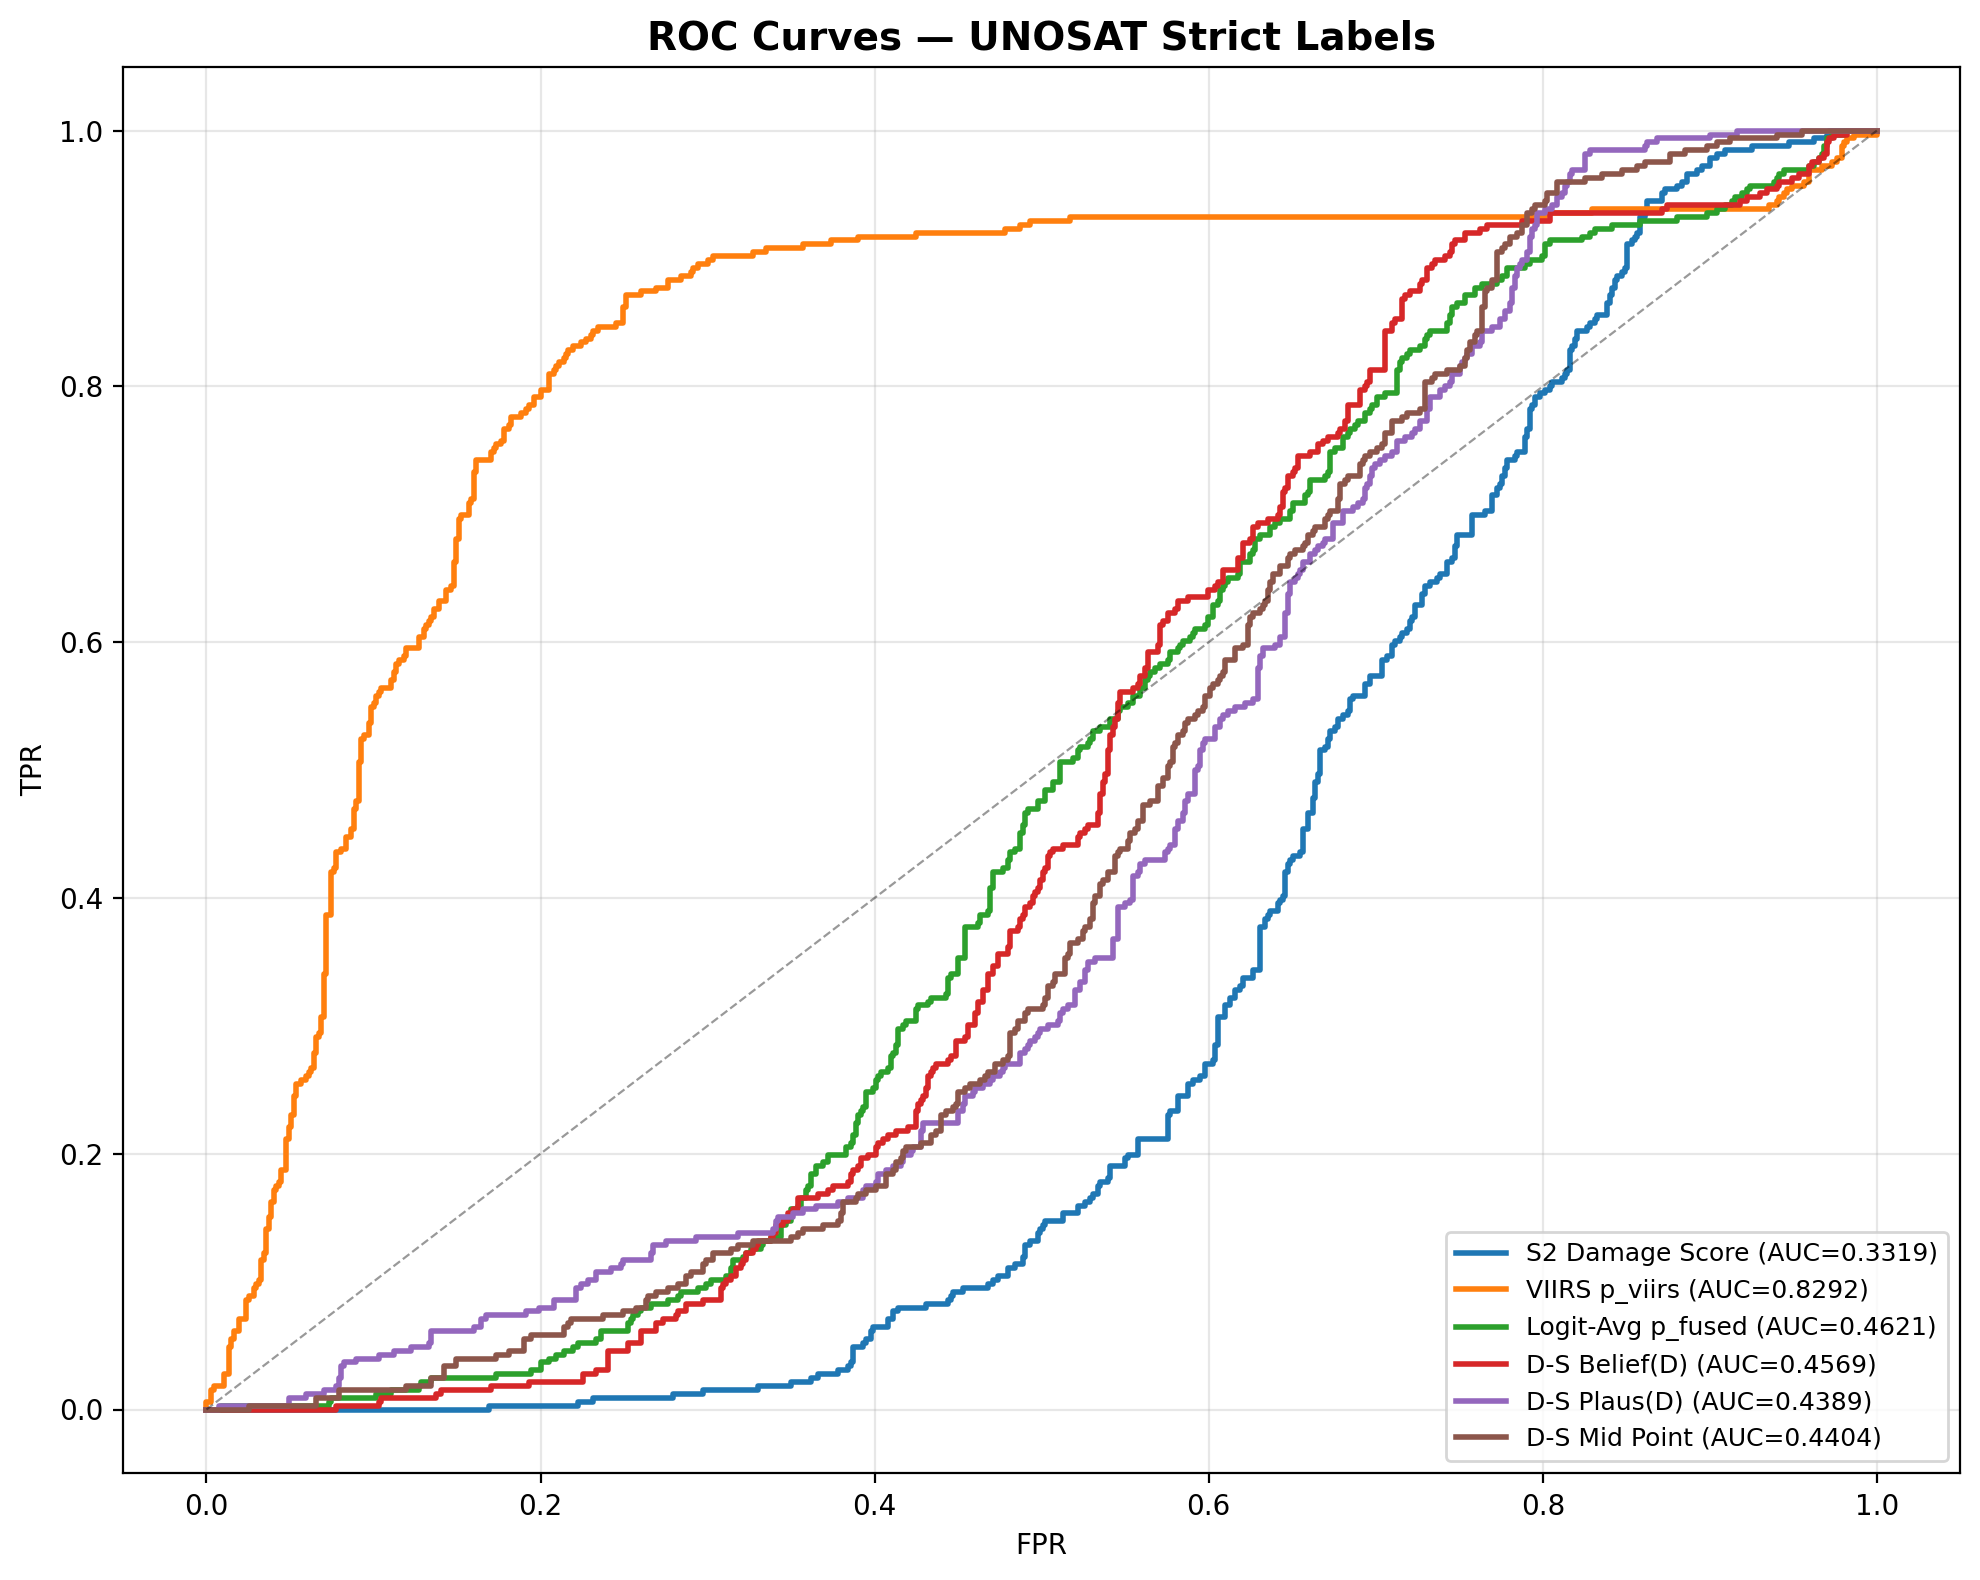
\includegraphics[width=0.85\textwidth]{figures/fig1_unosat_validation.png}
\caption{ROC and precision-recall curves for S2, VIIRS, logit-averaged
fusion, and D-S estimates evaluated against UNOSAT strict reference labels.
VIIRS shows stronger agreement with the UNOSAT reference labels
(AUC~$=0.829$) under this validation setting. The current S2-derived index
is weakly aligned (AUC~$=0.332$). Equal-weight fusion (AUC~$=0.462$) and
D-S-based scores (AUC~$0.44$--$0.46$) perform below VIIRS alone.}
\label{fig:unosat}
\end{center}
\end{figure}

Figure~\ref{fig:unosat} presents ROC and PR curves for all candidate scores
against the UNOSAT strict label set ($n=995$, $32.8\%$ positive). Three
patterns are immediately evident. First, VIIRS achieves AUC~$=0.829$
(Spearman $r=0.535$, Brier~$=0.222$), substantially outperforming the S2
index (AUC~$=0.332$, $r=-0.274$, Brier~$=0.343$) which falls below the
random-classifier baseline (AUC~$=0.5$). The S2 ROC curve lies almost
entirely below the diagonal, and its PR curve is essentially flat near the
prevalence baseline ($0.328$), indicating that the current S2-derived index
provides virtually no discriminative power for the specific building damage
types annotated in UNOSAT.

Second, all fusion-based scores---logit-averaged fusion (AUC~$=0.462$),
D-S belief (AUC~$=0.457$), D-S plausibility (AUC~$=0.439$), and D-S
midpoint (AUC~$=0.440$)---perform below VIIRS alone. Combining S2 with
VIIRS degrades rather than improves discriminative performance because the
S2 signal, which is weakly and negatively correlated with the UNOSAT
labels, introduces noise into the fused score. This is the first piece of
evidence that sensor disagreement, when unresolved, harms downstream
classification under a single-score aggregation.

Third, the PR curves reveal that none of the methods achieve high precision
at meaningful recall levels: the maximum F1 score is $0.630$ (VIIRS,
threshold~$=0.66$). This is expected---UNOSAT labels only a subset of
damage types (visible structural damage to buildings), and both S2 and
VIIRS register signals that extend beyond this narrow definition. The
validation thus benchmarks relative alignment rather than absolute accuracy.

\subsection{Bayesian Hierarchical Posterior}

\begin{table}[htp]
\centering
\caption{Bayesian hyperparameter posterior estimates. All parameters
converged with $\hat{R} < 1.01$ and 1 divergence in 4{,}000 draws.}
\label{tab:bayes_params}
\begin{tabular}{@{}lrrrrr@{}}
\toprule
\textbf{Parameter} & \textbf{Mean} & \textbf{SD} & \textbf{2.5\%} & \textbf{97.5\%} & \textbf{$\hat{R}$} \\
\midrule
$\mu$ (population mean, logit)        & $-1.695$ & $0.042$ & $-1.781$ & $-1.613$ & $1.000$ \\
$\tau$ (between-grid heterogeneity)   & $ 0.063$ & $0.047$ & $ 0.004$ & $ 0.172$ & $1.000$ \\
$\sigma_{\text{S2}}$ (S2 noise)       & $ 2.685$ & $0.059$ & $ 2.575$ & $ 2.803$ & $1.000$ \\
$\sigma_{\text{VIIRS}}$ (VIIRS noise) & $ 0.904$ & $0.018$ & $ 0.869$ & $ 0.940$ & $1.000$ \\
$\delta_{\text{S2}}$ (S2 bias)        & $-1.705$ & $0.042$ & $-1.789$ & $-1.624$ & $1.000$ \\
\bottomrule
\end{tabular}
\end{table}

\begin{figure}[htp]
\begin{center}
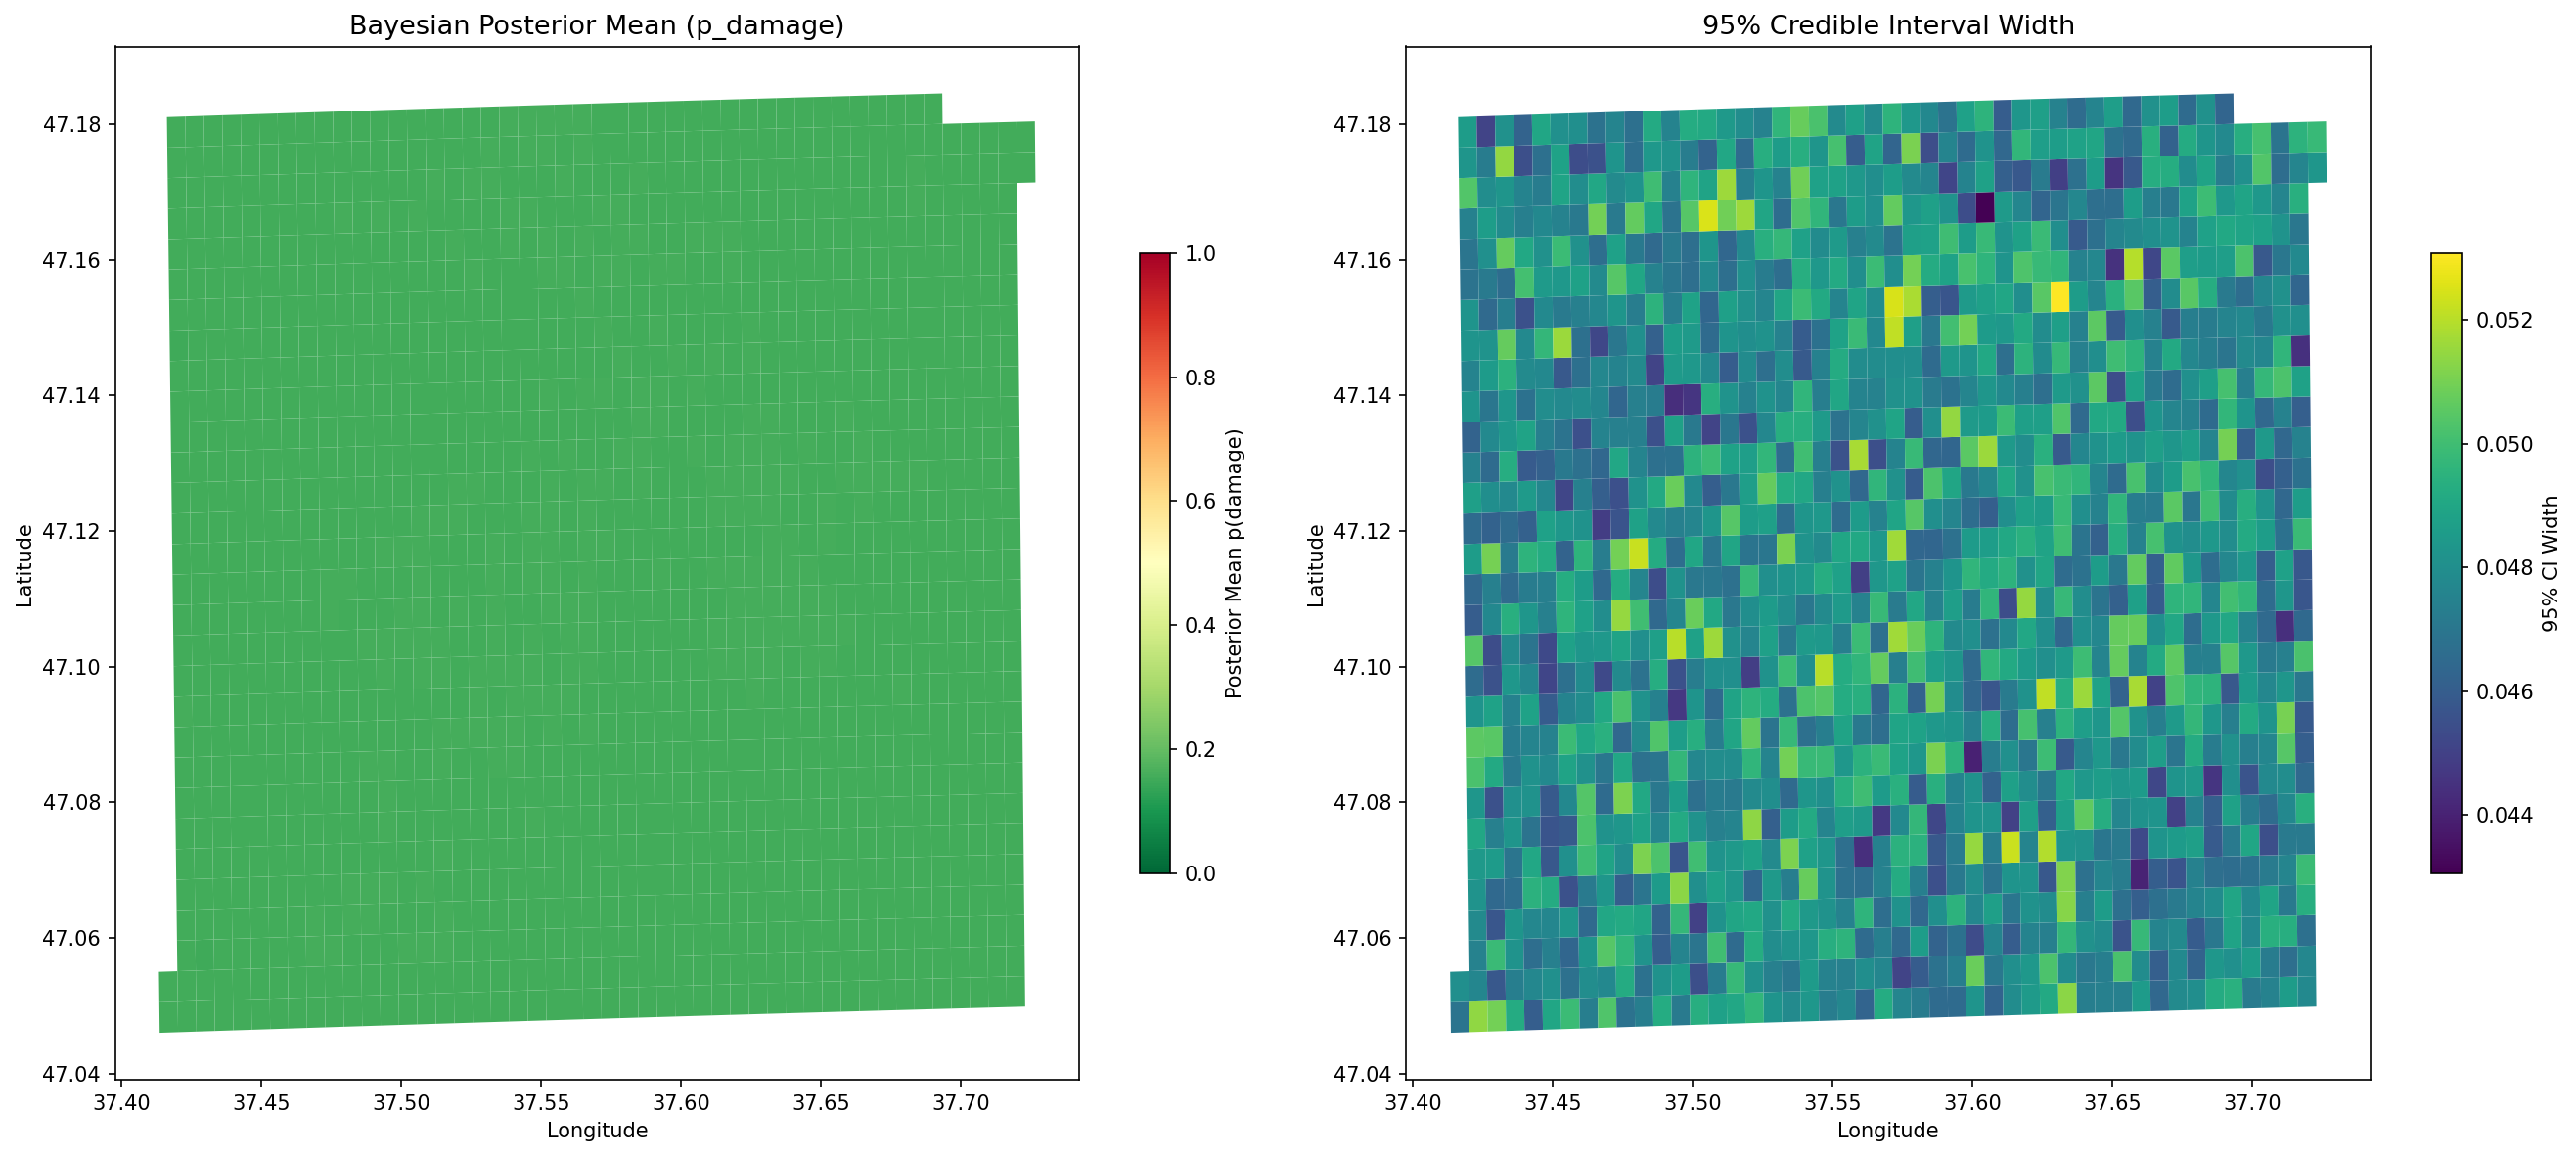
\includegraphics[width=0.48\textwidth]{figures/fig2_bayesian_posterior_map.png}
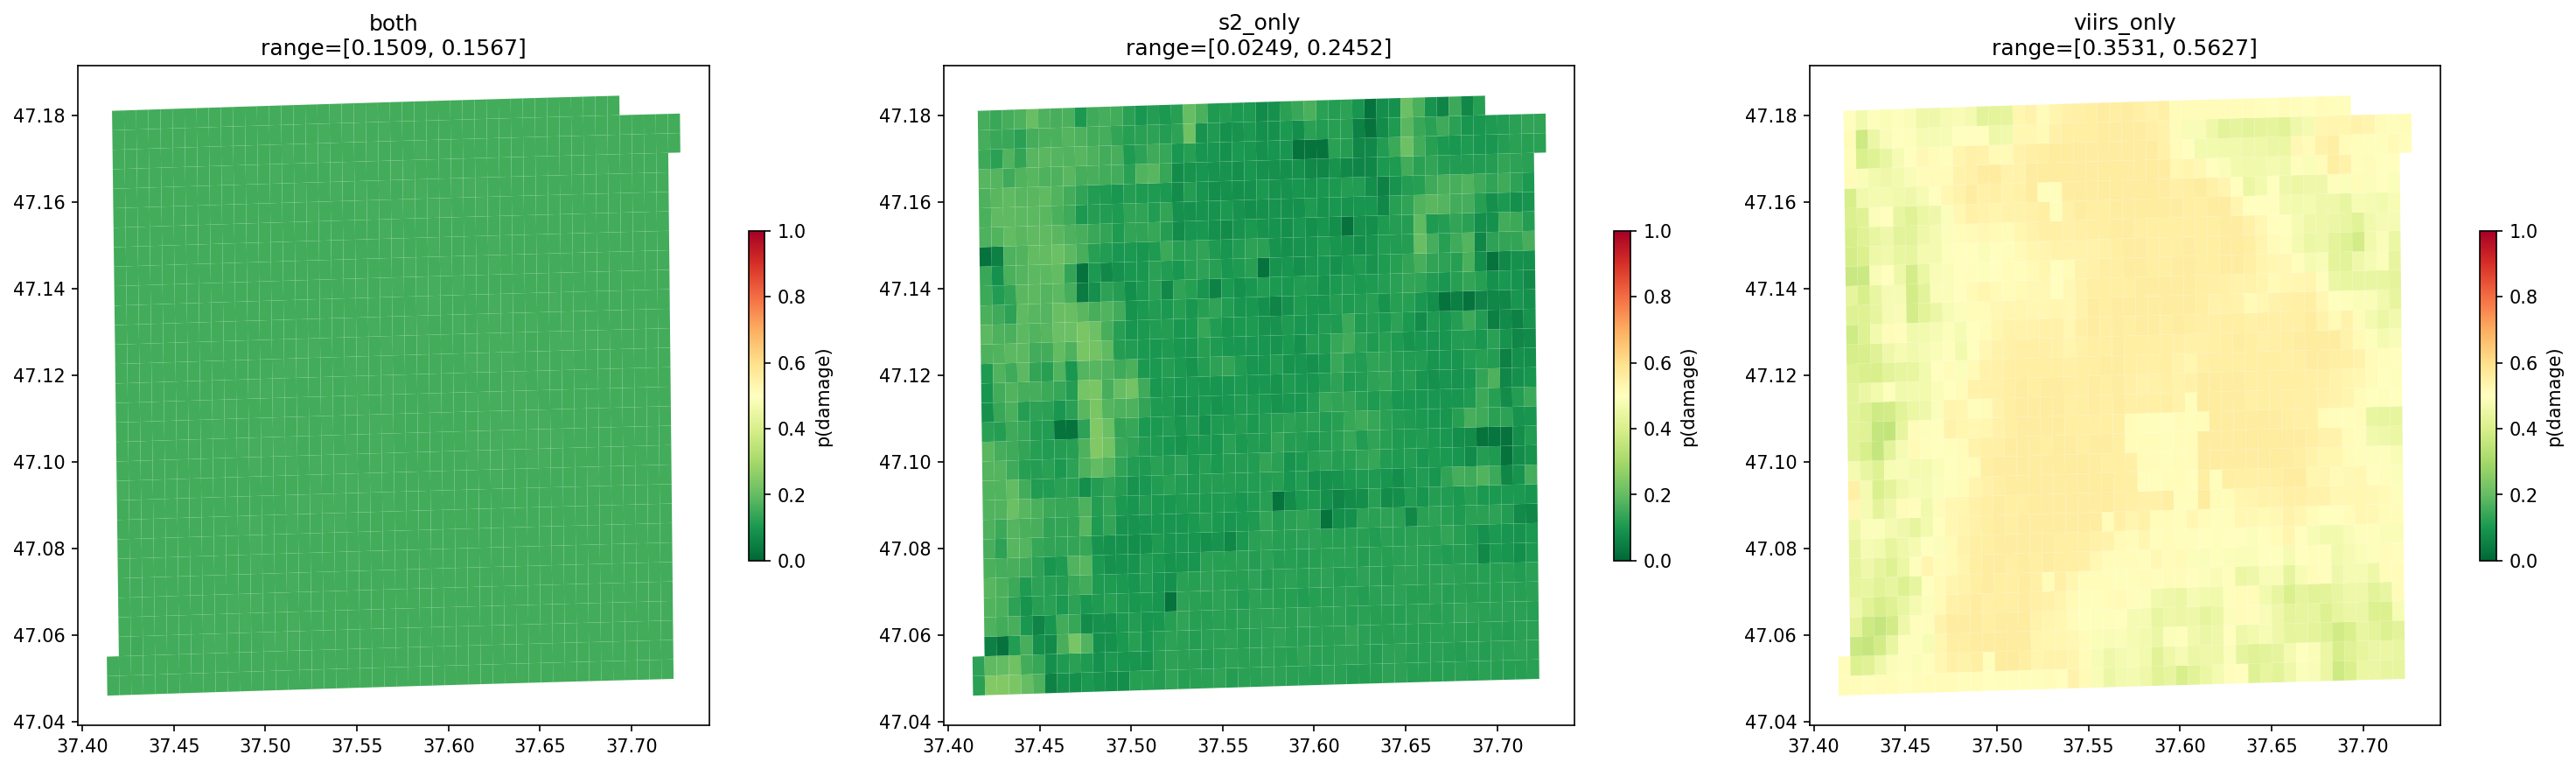
\includegraphics[width=0.48\textwidth]{figures/fig3_sensor_only_comparison.png}
\caption{\textbf{(Left)} Bayesian posterior mean damage probability map.
The posterior is near-uniform ($p_i \in [0.151, 0.157]$) across all 1{,}380
grids. \textbf{(Right)} Sensor-only posterior comparison: the S2-only model
produces $p \in [0.025, 0.245]$, VIIRS-only produces $p \in [0.353, 0.563]$,
while the joint model collapses to $p \in [0.151, 0.157]$.}
\label{fig:bayes_maps}
\end{center}
\end{figure}

Table~\ref{tab:bayes_params} reports the Bayesian hyperparameter posterior
estimates from the joint model. Three parameter estimates jointly explain
why the fused posterior collapses. First, $\tau = 0.063$ (95\% CI:
$[0.004, 0.172]$) indicates that the joint data provide essentially no
support for shared grid-level heterogeneity after accounting for sensor
bias and noise. This is the formal statistical statement of the claim that
S2 and VIIRS cannot be reconciled into a single latent damage state:
if they could, $\tau$ would be substantially larger, reflecting genuine
between-grid variation in the common damage probability.

Second, the estimated sensor noise $\sigma_{\text{S2}} = 2.685$ is
approximately $3\times$ larger than $\sigma_{\text{VIIRS}} = 0.904$ on the
logit scale. The model thus learns that S2 observations are substantially
less precise than VIIRS observations. In a hierarchical model without
external validation, the noisier sensor receives less weight in determining
the latent state.

Third, the systematic bias $\delta_{\text{S2}} = -1.705$ captures the
directional nature of the disagreement: S2 consistently reports damage
probabilities approximately $1.7$ logit units below the latent state.
Equivalently, after correcting for this bias, the adjusted S2 and VIIRS
signals share a common location, but the large $\sigma_{\text{S2}}$ means
the S2 contribution to the posterior is heavily regularized.

Figure~\ref{fig:bayes_maps} makes the practical consequence of these
parameter estimates visually stark. The left panel shows the joint
posterior mean map: a near-uniform field of $p_i \approx 0.155$ across all
1{,}380 grids, with the entire AOI spanning only $[0.151, 0.157]$. This
map is essentially uninformative for spatial damage triage---it assigns the
same moderate damage probability regardless of whether a grid contains a
destroyed city block or an intact agricultural field.

The right panel reveals that this uniformity is an artifact of fusion, not
of data poverty. The S2-only posterior (top row) spans $[0.025, 0.245]$
(22 percentage points), with elevated probabilities concentrated in the
urban core and industrial zones where structural damage is visually
evident. The VIIRS-only posterior (bottom row) spans $[0.353, 0.563]$ (21
percentage points), with high values distributed across both urban and
peri-urban areas---consistent with widespread power and activity loss.
These are two different and spatially informative maps. The joint model
(bottom of the right panel) collapses both into a single, spatially
invariant value. We note that single-sensor MCMC diagnostics were weaker
(S2-only: 263 divergences, $\hat{R}_{\max}=1.21$; VIIRS-only: 122
divergences, $\hat{R}_{\max}=1.35$) than the joint model, so single-sensor
posterior ranges should be interpreted as diagnostic comparisons rather
than precise uncertainty estimates.

\subsection{KLD/JSD Information Gain and Fusion Suppression}

\begin{table}[htp]
\centering
\caption{KLD/JSD information gain summary (nats). All metrics computed at
the Bernoulli probability level with neutral prior $p=0.5$.}
\label{tab:kld}
\begin{tabular}{@{}lrrrr@{}}
\toprule
\textbf{Metric} & \textbf{Mean} & \textbf{Median} & \textbf{Min} & \textbf{Max} \\
\midrule
KL(S2 $\|$ neutral)          & 0.496 & 0.501 & 0.301 & 0.591 \\
KL(VIIRS $\|$ neutral)       & 0.007 & 0.006 & 0.000 & 0.072 \\
KL(Both $\|$ neutral)        & 0.261 & 0.261 & 0.259 & 0.269 \\
KL(S2 $\|$ S2 global)        & 0.003 & 0.001 & 0.000 & 0.050 \\
KL(VIIRS $\|$ VIIRS global)  & 0.007 & 0.005 & 0.000 & 0.075 \\
$\mathbf{KL(Both \| Both_{global})}$ & $\mathbf{\approx 0}$ & $\mathbf{\approx 0}$ & $\mathbf{\approx 0}$ & $\mathbf{<0.001}$ \\
JSD(S2, VIIRS)               & 0.146 & 0.150 & 0.053 & 0.212 \\
Fusion KL loss               & 0.235 & 0.240 & 0.041 & 0.329 \\
Fusion suppression ratio     & 0.468 & 0.479 & 0.137 & 0.557 \\
\bottomrule
\end{tabular}
\end{table}

\begin{figure}[htp]
\begin{center}
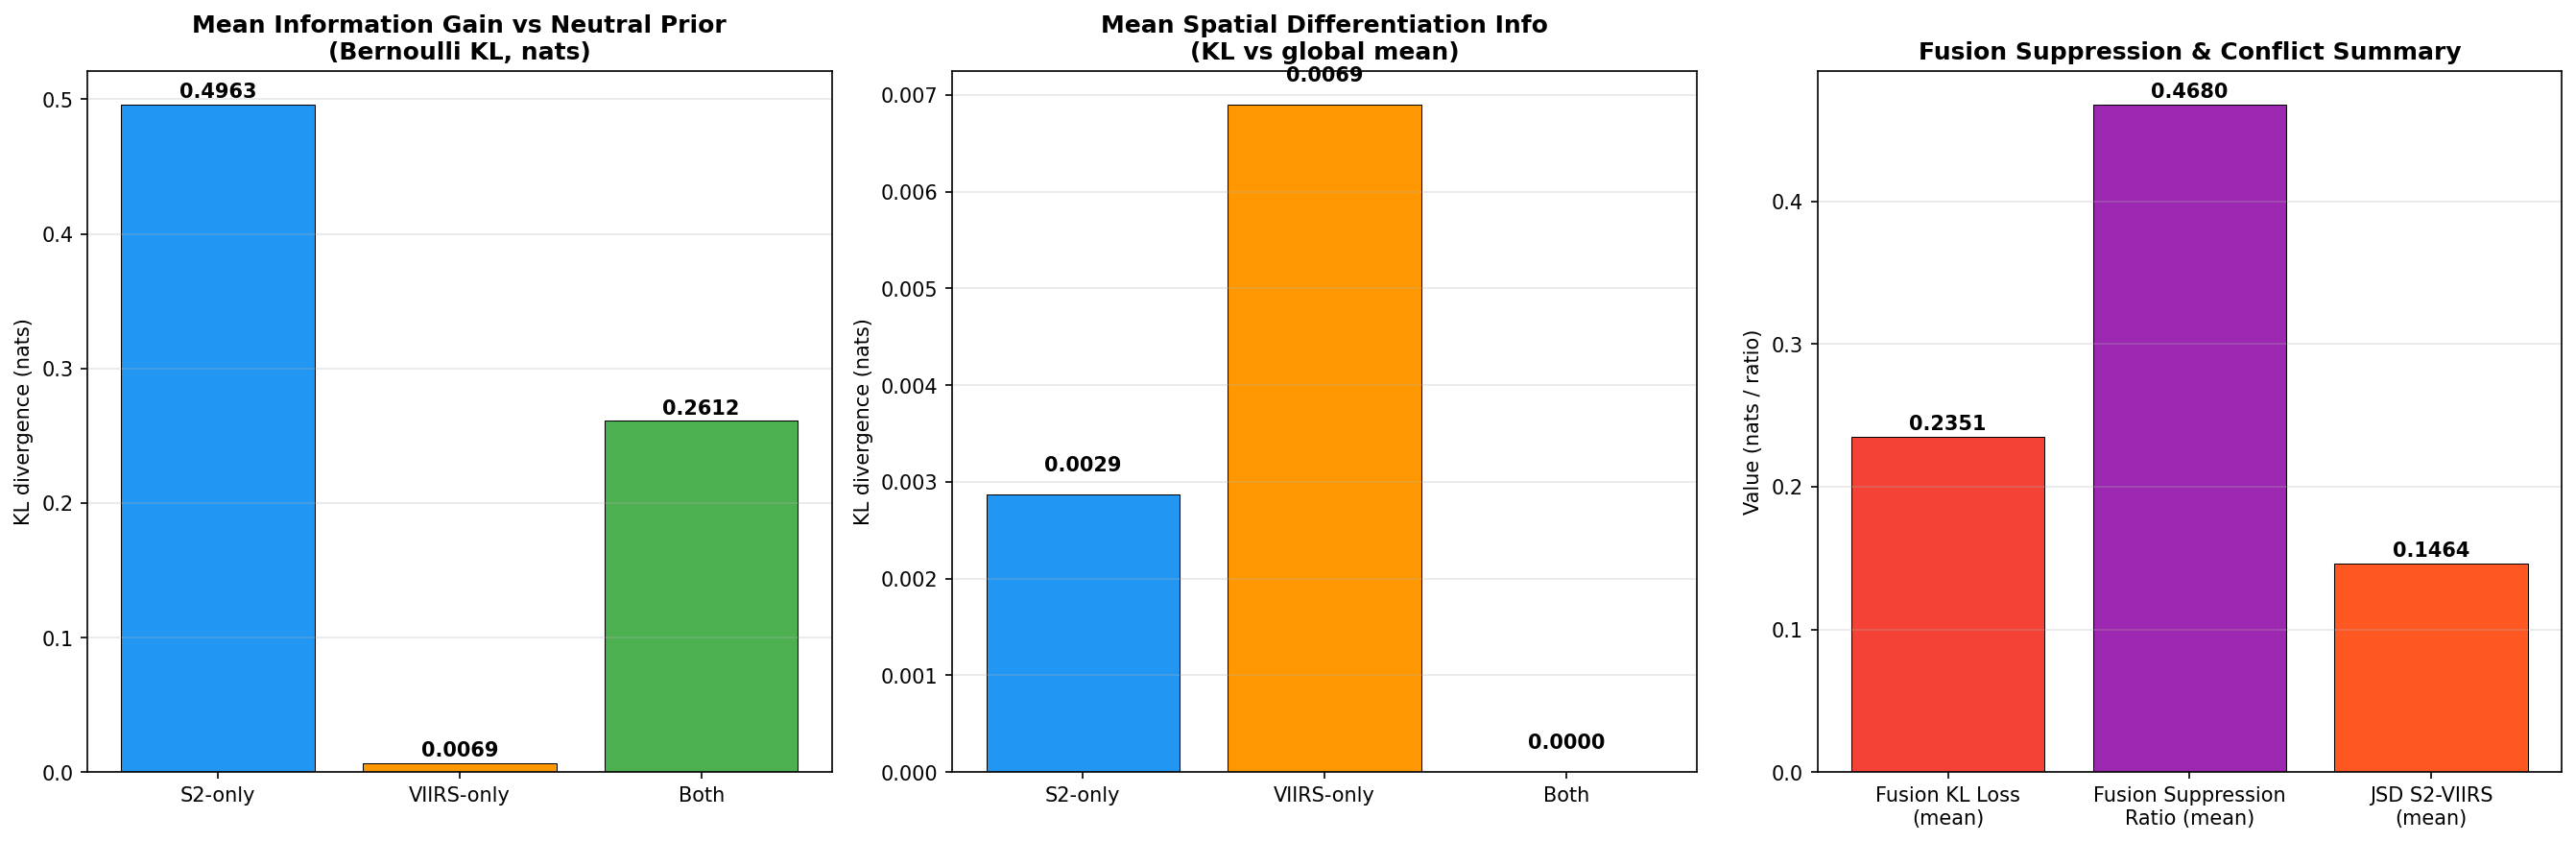
\includegraphics[width=0.48\textwidth]{figures/fig4_kld_barplot.png}
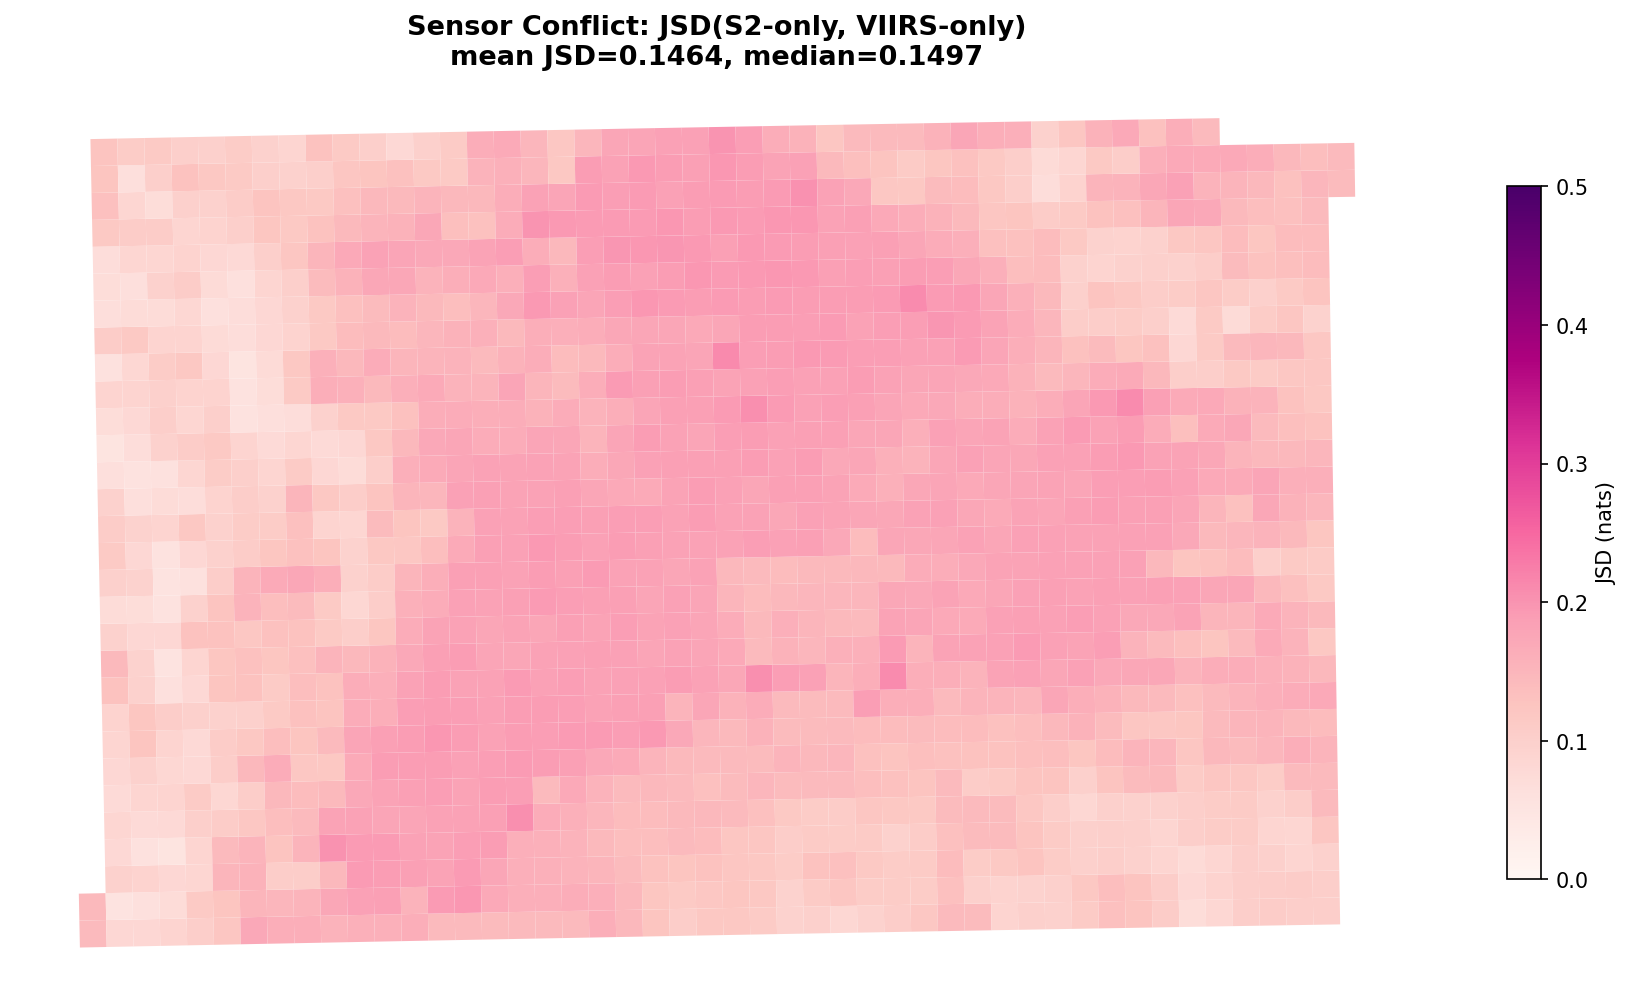
\includegraphics[width=0.48\textwidth]{figures/fig5_jsd_conflict_map.png}
\caption{\textbf{(Left)} KLD summary barplot: S2 deviates strongly from the
neutral prior ($p=0.05$ vs.\ $p=0.5$), VIIRS remains near neutral, and the
fused posterior falls in between. Spatial differentiation (KL vs.\ global
mean) is near zero for the fused model. \textbf{(Right)} JSD(S2, VIIRS)
conflict map: all 1{,}380 grids exhibit moderate to high sensor conflict
(JSD~$\in [0.053, 0.212]$ nats).}
\label{fig:kld}
\end{center}
\end{figure}

\begin{figure}[htp]
\begin{center}
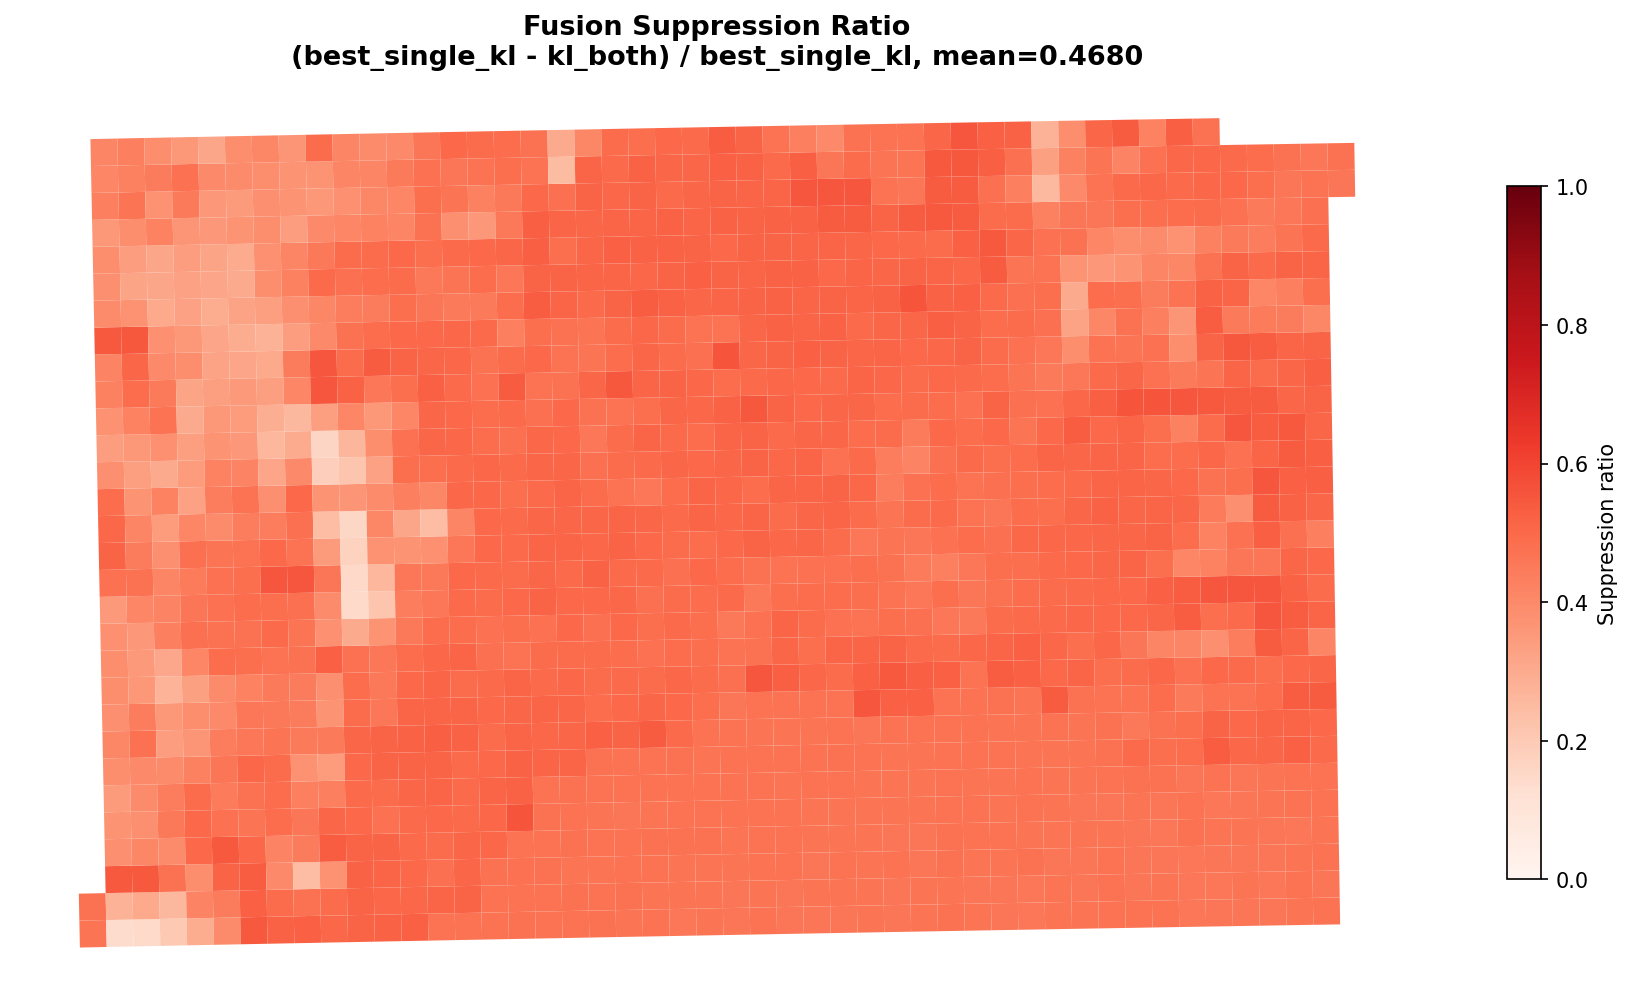
\includegraphics[width=0.7\textwidth]{figures/fig6_fusion_suppression_map.png}
\caption{Fusion suppression ratio map. Values near 0.5 indicate that
approximately half of the best single-sensor information is suppressed in
the fused posterior. The suppression is spatially widespread, reflecting the
systematic nature of the S2-VIIRS disagreement.}
\label{fig:suppression}
\end{center}
\end{figure}

Table~\ref{tab:kld} and Figures~\ref{fig:kld}--\ref{fig:suppression}
present the quantitative information decomposition. The barplot
(Figure~\ref{fig:kld}, left) reveals an asymmetry that is central to
understanding the fusion dynamics. The blue bar shows KL(S2 $\|$
neutral)~$=0.496$ nats---a large divergence driven by the S2-only
posterior being concentrated near $p \approx 0.05$, far from the neutral
prior of $0.5$. The orange bar shows KL(VIIRS $\|$ neutral)~$=0.007$
nats---a negligible divergence because the VIIRS-only posterior mean is
approximately $0.50$, very close to the neutral prior. The green bar
(KL(Both $\|$ neutral)~$=0.261$ nats) falls between the two, reflecting
the fused posterior at $p \approx 0.155$.

This pattern has a specific interpretation. The KL vs.\ neutral prior
measures how far a posterior moves us from complete uncertainty ($p=0.5$).
S2 produces a large movement (toward ``probably not damaged''), VIIRS
produces almost no movement (it remains near ``completely uncertain'' on
average), and the fused model lands in between. Critically, this metric
does \emph{not} measure which sensor is ``better''---it measures which
sensor deviates more from a uniform prior, which is a function of the
sensor's calibration rather than its accuracy.

The spatial differentiation bars (gray, Figure~\ref{fig:kld}, left) tell a
different and more diagnostic story. KL(S2 $\|$ S2$_{\text{global}}$)
$=0.003$ nats and KL(VIIRS $\|$ VIIRS$_{\text{global}}$) $=0.007$ nats
confirm that each single-sensor posterior retains measurable grid-to-grid
variation (VIIRS slightly more than S2). But KL(Both $\|$
Both$_{\text{global}}$) $\approx 0$ nats---three orders of magnitude
smaller---confirms that spatial differentiation is essentially eliminated
under the joint model. This is not a marginal effect; it is a near-total
collapse.

The JSD conflict map (Figure~\ref{fig:kld}, right) shows that this
collapse is driven by pervasive sensor disagreement. Every one of the
1{,}380 grids has JSD(S2, VIIRS) $> 0.05$ nats, with a mean of $0.146$
and a maximum of $0.212$. The spatial pattern is instructive: conflict is
highest in the urban core and industrial periphery, where S2 detects strong
spectral change (rubble, exposed soil) but VIIRS detects only moderate NTL
loss (partial power retention), or vice versa. No grid exhibits low
conflict; this is a systematic, AOI-wide phenomenon, not an artifact of a
few outlier cells.

The fusion suppression map (Figure~\ref{fig:suppression}) translates this
conflict into an information-loss metric. The suppression ratio---the
fraction of the best single-sensor's KL that is lost in fusion---averages
$46.8\%$ (median $47.9\%$) and ranges from $13.7\%$ to $55.7\%$. The map
shows that suppression is spatially pervasive: red and orange tones (high
suppression) dominate the entire AOI, with only small pockets of lower
suppression near the edges. This uniformity confirms that the information
loss is not driven by a few anomalous grids but by the systematic
incompatibility of the S2 and VIIRS spatial patterns across the entire
study area.

\subsection{Bayesian vs.\ Dempster-Shafer Consistency}

\begin{table}[htp]
\centering
\caption{Bayesian vs.\ D-S consistency classification. Genuine agreement
requires the D-S interval to be narrow (below the 75th percentile of D-S
interval width); uncertainty-compatible refers to wide D-S intervals that
coincidentally cover the Bayesian mean.}
\label{tab:consistency}
\begin{tabular}{@{}lrrrr@{}}
\toprule
\textbf{Consistency Label} & \textbf{$N$} & \textbf{\%} &
  \textbf{Mean JSD} & \textbf{Mean D-S Width} \\
\midrule
Genuine agreement        & 689 & 49.9 & 0.153 & 0.197 \\
Uncertainty-compatible   & 141 & 10.2 & 0.166 & 0.277 \\
Weak consistent          & 128 &  9.3 & 0.148 & 0.216 \\
Divergent (low Bayes)    & 360 & 26.1 & 0.128 & 0.300 \\
Divergent (high Bayes)   &  28 &  2.0 & 0.124 & 0.093 \\
No D-S data              &  34 &  2.5 & ---   & ---   \\
\midrule
\textbf{Total}           & \textbf{1{,}380} & \textbf{100.0} & \textbf{0.146} & \textbf{0.225} \\
\bottomrule
\end{tabular}
\end{table}

\begin{figure}[htp]
\begin{center}
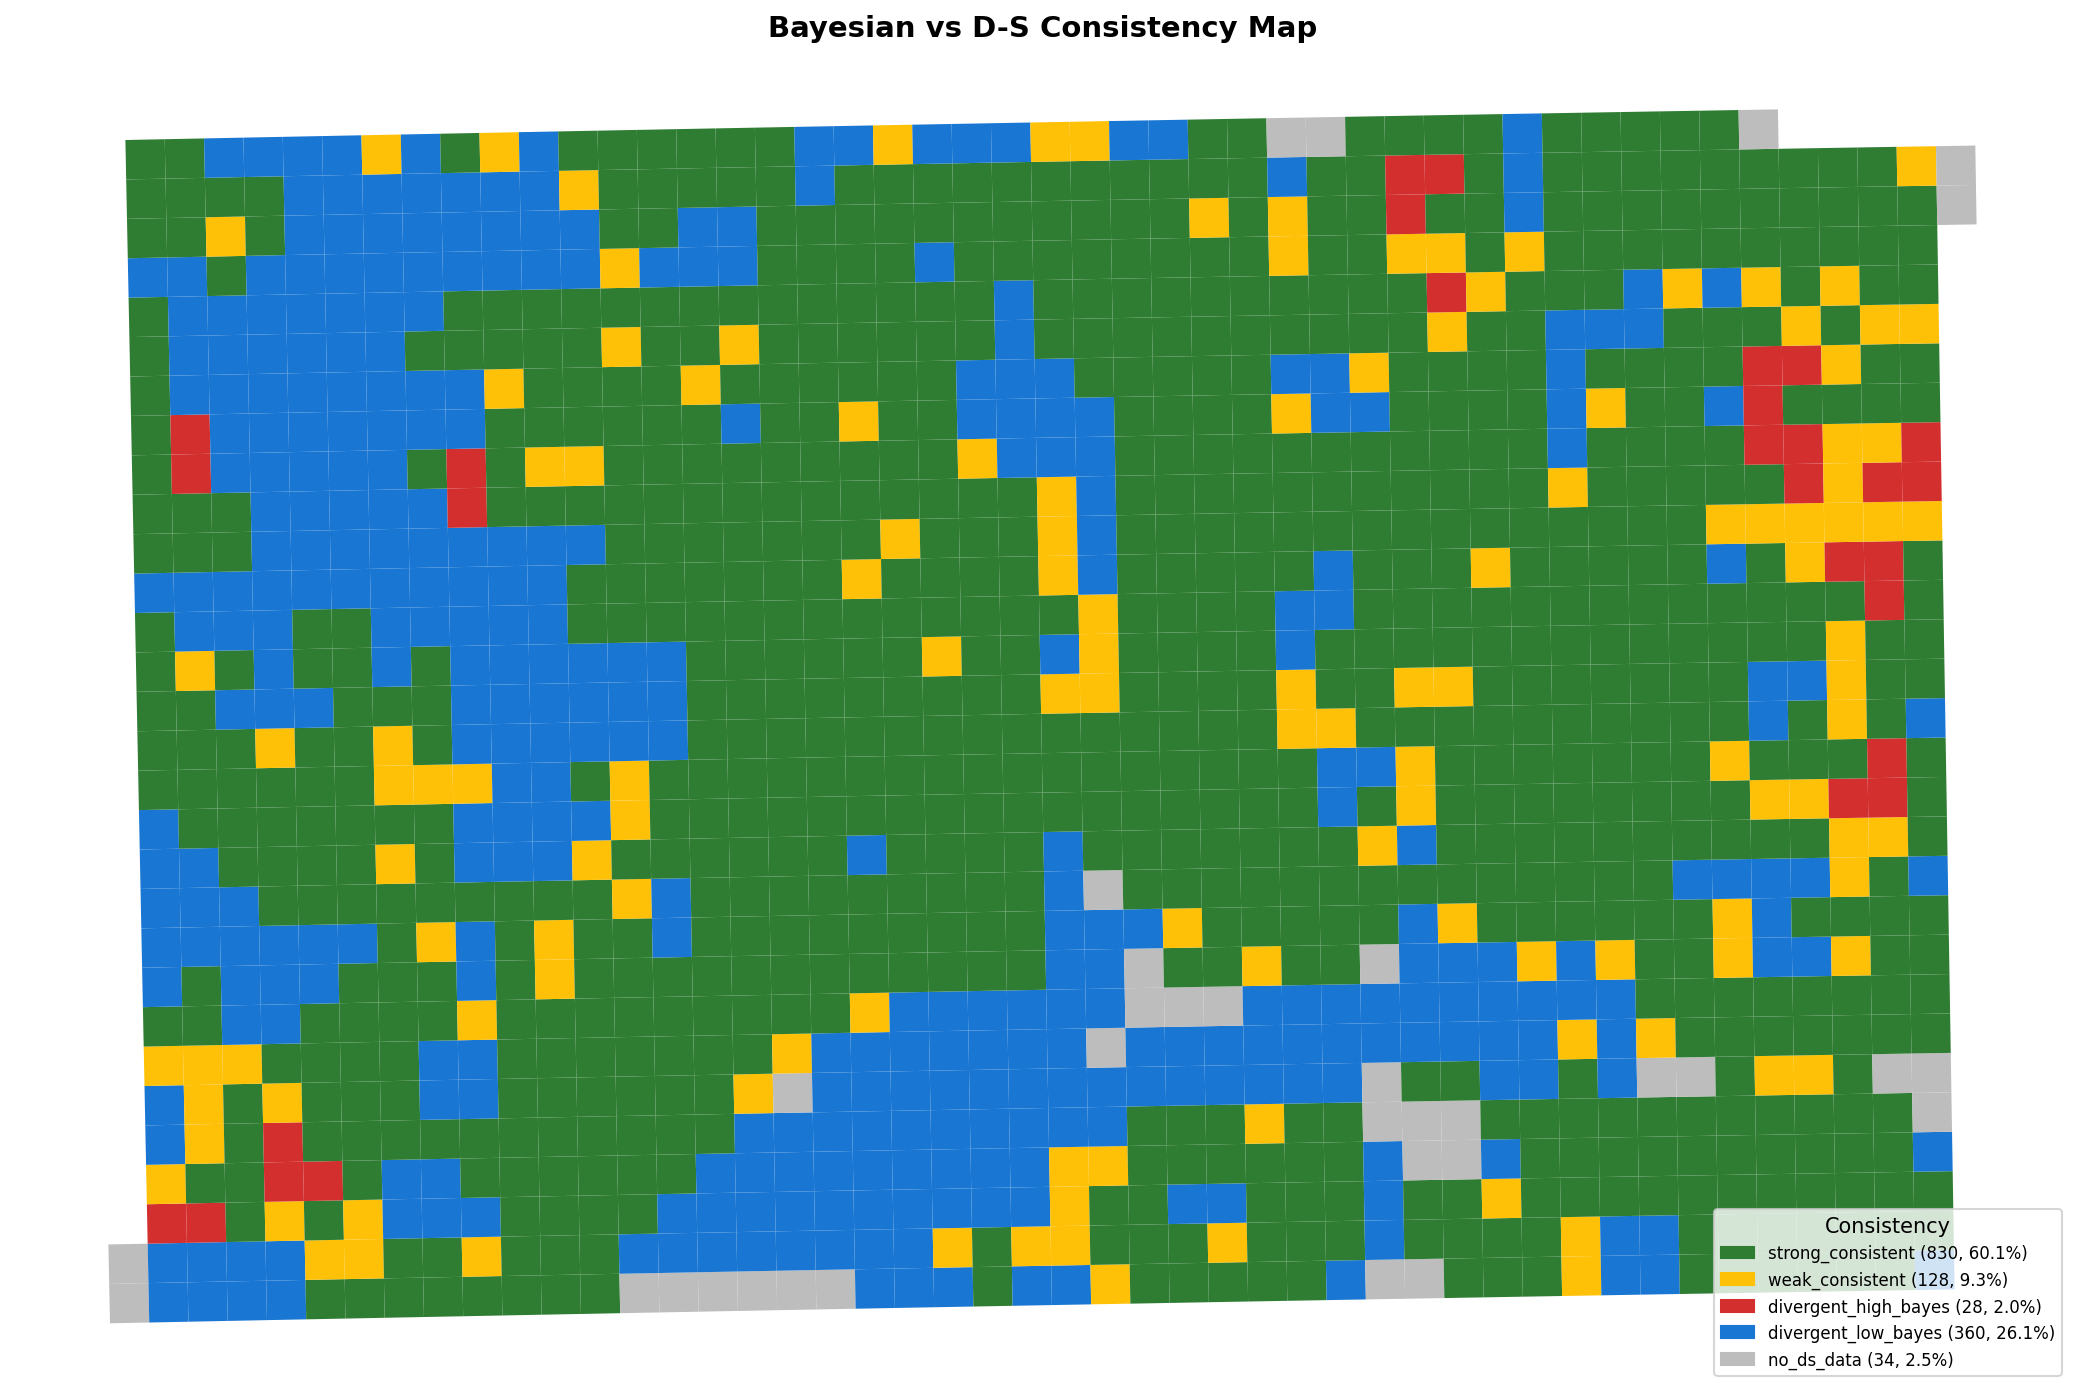
\includegraphics[width=0.7\textwidth]{figures/fig7_consistency_map.png}
\caption{Bayesian vs.\ D-S consistency map. Green: genuine agreement
($49.9\%$); yellow: uncertainty-compatible ($10.2\%$); orange: weak
consistent ($9.3\%$); red/blue: divergent ($28.1\%$). The divergence
is predominantly of the ``divergent\_low\_bayes'' type, where the
Bayesian posterior mean lies below the D-S belief lower bound.}
\label{fig:consistency}
\end{center}
\end{figure}

\begin{figure}[htp]
\begin{center}
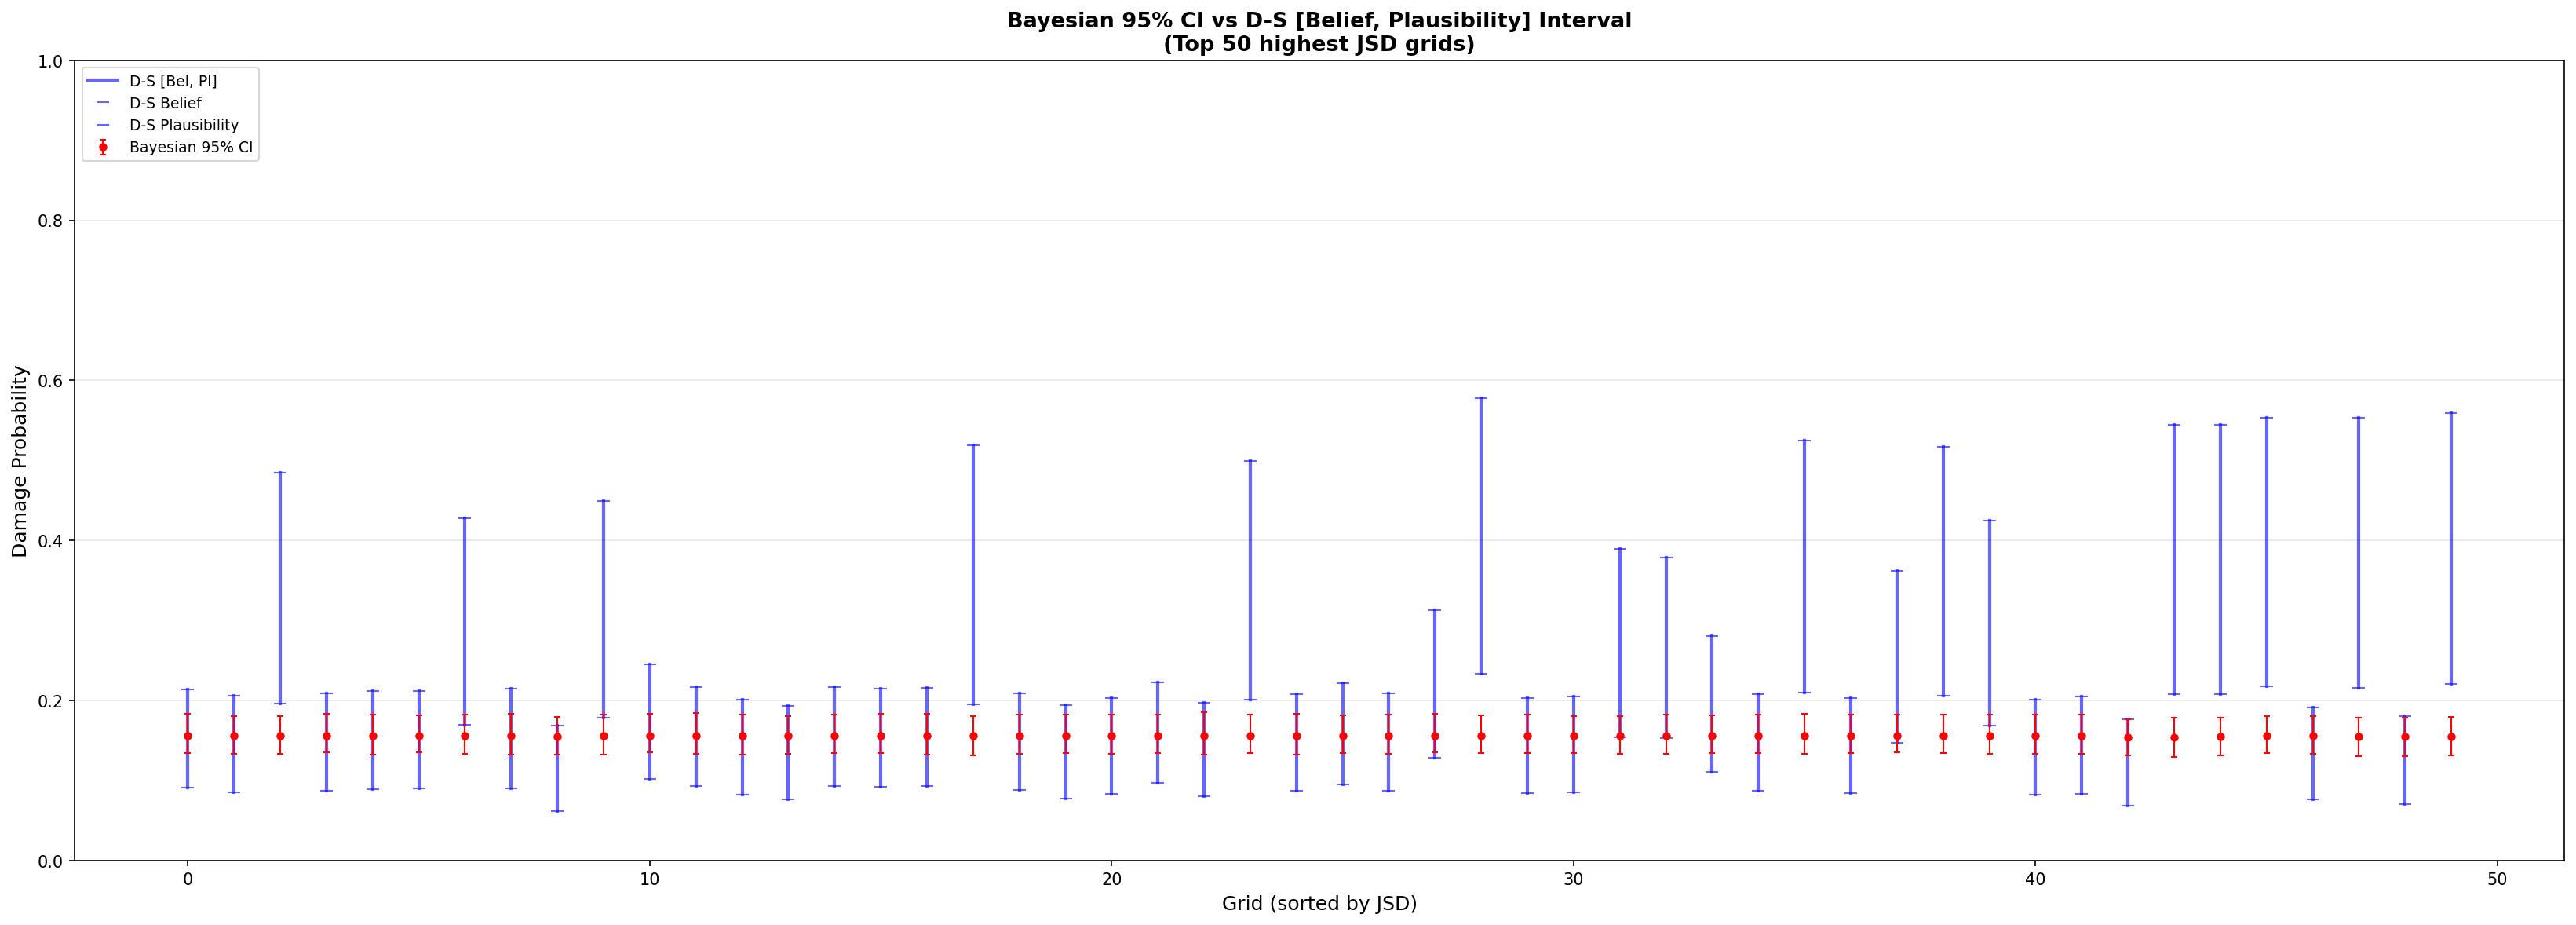
\includegraphics[width=0.85\textwidth]{figures/fig8_interval_comparison.png}
\caption{Bayesian 95\% credible intervals vs.\ D-S [Belief, Plausibility]
intervals for the 50 grids with highest JSD. Red dots: Bayesian posterior
means with error bars. Blue lines: D-S intervals.}
\label{fig:interval}
\end{center}
\end{figure}

Table~\ref{tab:consistency} and Figures~\ref{fig:consistency}--\ref{fig:interval}
provide the grid-level comparison between the two fusion paradigms.

The consistency map (Figure~\ref{fig:consistency}) reveals a spatially
structured pattern. Green grids (genuine agreement, $49.9\%$) are
distributed broadly across the AOI but concentrated in areas where both
sensors provide moderate evidence and the D-S interval is relatively narrow
(below the 75th percentile of interval width, $0.184$). In these grids, the
Bayesian posterior mean ($\approx 0.155$) and the D-S belief/plausibility
interval agree that the damage evidence is inconclusive but bounded.
Yellow grids (uncertainty-compatible, $10.2\%$) appear more scattered; here
the D-S interval is wide enough ($>0.184$) that it mechanically covers the
Bayesian mean even though the two estimates are not genuinely aligned.
These grids represent a non-trivial fraction of what would naively be
called ``consistent''---without the width-based sub-classification, the
apparent agreement rate would be misleadingly inflated.

Red and blue grids (divergent, $28.1\%$) show a striking spatial
concentration in the urban core and eastern industrial zone. The divergence
is overwhelmingly of the ``divergent\_low\_bayes'' type ($26.1\%$): the
Bayesian posterior mean lies entirely \emph{below} the D-S belief lower
bound. For these grids, D-S concludes ``probably damaged'' (belief $>0.3$,
often $>0.5$) while the Bayesian model concludes ``probably not damaged''
($p \approx 0.155$). The ``divergent\_high\_bayes'' type ($2.0\%$)---where
Bayesian is above D-S plausibility---is negligible.

The interval comparison plot (Figure~\ref{fig:interval}) explains the
mechanism behind this divergence, using the 50 grids with the highest
JSD. Each vertical blue line spans a D-S [Belief, Plausibility] interval;
each red dot with error bar is a Bayesian posterior mean with its 95\%
credible interval. Two features stand out. First, the D-S intervals are
consistently wider than the Bayesian CIs---mean D-S width $0.225$ vs.\
mean Bayesian CI width $0.048$---reflecting the fundamentally different
uncertainty representations: D-S expresses ignorance through interval
width, while the Bayesian model concentrates uncertainty in the
hyperparameters and produces narrow grid-level CIs after shrinkage.

Second, the Bayesian estimates are systematically lower than the D-S
belief bounds for most of these high-conflict grids. This is because D-S
combines BPA masses without hierarchical regularization: when one sensor
provides strong evidence for damage (e.g., S2 with raw $p_{\text{S2}}
>0.7$), the combined belief rises accordingly, regardless of that sensor's
global reliability. The Bayesian model, having learned that S2 is noisy
($\sigma_{\text{S2}} = 2.685$), shrinks these high values toward the
population mean. Relative to the UNOSAT external reference, approximately
$60\%$ of the divergent\_low\_bayes grids are labeled as undamaged by
UNOSAT, suggesting that the Bayesian shrinkage, while arguably too
aggressive, is directionally consistent with the external reference in a
majority of these cases.

A counterintuitive pattern completes the picture: JSD and Bayesian-D-S
distance are \emph{negatively} correlated ($r = -0.35$). Grids with the
highest sensor conflict tend to have the \emph{smallest} distance between
the Bayesian and D-S estimates. The reason is mechanical: high conflict
produces wide D-S intervals (because Dempster's rule assigns mass to the
conflict term $K$), and wide intervals are more likely to encompass the
Bayesian mean. The true divergence between the paradigms is concentrated
in grids where sensor evidence is locally consistent (low JSD, narrow D-S
interval) but the Bayesian model's global shrinkage pulls the estimate away
from the D-S interval. This is where the philosophical difference between
the two approaches---global regularization vs.\ local evidence
combination---manifests most clearly.

%=====================================================================
\section{Discussion}\label{sec:discussion}

\subsection{Sensor Conflict Is Not Sensor Failure}

The S2 and VIIRS damage indices disagree systematically across the Mariupol
AOI because they respond to different physical manifestations of conflict
damage. S2 spectral change detects surface alteration---exposed rubble,
soil disturbance, vegetation removal---that may or may not correspond to
building destruction. VIIRS NTL loss detects reduced human activity, which
can arise from structural damage, power grid failure, or population
displacement. A structurally intact but unlit building (power outage) and a
demolished building near a functioning streetlight produce opposite
sensor signatures. These are not measurement errors but genuine
physical phenomena captured by different sensing modalities.

The JSD analysis confirms that every grid in the AOI exhibits
non-negligible sensor conflict (JSD~$>0.05$ nats). This pervasive
disagreement is a feature of the data, not a failure of either sensor.
We therefore caution against interpreting the UNOSAT validation results
as evidence that ``VIIRS is better than S2.'' Rather, VIIRS shows stronger
agreement with the UNOSAT reference labels under this specific validation
setting, and the current S2-derived index may be more sensitive to a
different damage dimension not captured by the UNOSAT classification scheme.

\subsection{Limits of the Single Latent State Assumption}

Under the single latent state assumption (Equation~\ref{eq:L1}--\ref{eq:L3}),
the Bayesian model interprets systematic disagreement as sensor bias
($\delta_{\text{S2}}=-1.70$) and noise ($\sigma_{\text{S2}}=2.69$). The
model's response is rational: when two information sources systematically
disagree and neither is externally validated, the only coherent Bayesian
update is to increase uncertainty and shrink toward the prior. The resulting
posterior is internally coherent but limited for spatial discrimination,
producing $p_i \approx 0.155$ for every grid.

The small $\tau=0.063$ confirms that the joint data provide essentially no
support for shared grid-level heterogeneity after accounting for sensor bias
and noise. The sensor-only baselines demonstrate that this is not because
the individual sensors lack spatial information, but because their spatial
patterns are inconsistent with a shared latent state.

\subsection{When Multi-Sensor Fusion Improves Estimation}

The fusion suppression ratio of $46.8\%$ quantifies when adding a sensor
\emph{reduces} rather than increases usable information. This does not
imply that multi-sensor fusion is undesirable; rather, it identifies the
conditions under which fusion is beneficial: the sensors must measure
compatible dimensions of the target phenomenon, or the model must explicitly
accommodate multiple latent dimensions. In the present case, S2 and VIIRS
are better understood as measuring two distinct but correlated damage
dimensions---structural alteration and functional cessation---rather than
as noisy replicates of a single damage state.

\subsection{Toward a Multi-Dimensional Damage Model}

The comparison between Bayesian and D-S fusion paradigms clarifies the
trade-off. The Bayesian model provides a single coherent posterior but
sacrifices spatial discrimination when evidence conflicts. D-S preserves
uncertainty through wider intervals but may over-weight strong
single-sensor evidence in the absence of hierarchical shrinkage. Neither
approach is universally superior; they serve complementary roles.

A natural extension is a multi-dimensional latent damage model with
explicitly correlated structural and functional damage states. Each sensor
would primarily inform its corresponding dimension, with a correlation
structure allowing information sharing. This would preserve the spatial
information present in each individual sensor while still leveraging the
benefits of multi-source fusion.

%=====================================================================
\section{Limitations}\label{sec:limitations}

\begin{enumerate}
  \item \textbf{UNOSAT is an external reference, not absolute ground truth.}
    It captures visually identifiable building damage but may miss
    functional damage, sub-detection-threshold structural alteration, or
    damage types outside its classification scheme.
  \item \textbf{Single-sensor MCMC diagnostics were weaker than the joint
    model.} The S2-only and VIIRS-only Bayesian models showed elevated
    divergences and $\hat{R}$ values; their posterior ranges should be
    interpreted as diagnostic comparisons rather than precise single-sensor
    uncertainty estimates.
  \item \textbf{Results are conditional on the 500~m grid scale.} Different
    spatial resolutions would yield different conflict and information gain
    estimates due to aggregation effects.
  \item \textbf{Temporal mismatch.} The S2 and VIIRS pre/post pairs capture
    slightly different time windows, and damage processes evolve between
    acquisition dates.
  \item \textbf{The current S2 index is one of many possible formulations.}
    Alternative spectral indices, change detection algorithms, or
    texture-based features could produce different alignment with UNOSAT
    labels.
  \item \textbf{VIIRS NTL loss conflates multiple processes.} Reduced NTL
    can reflect building destruction, power grid damage, population
    displacement, or deliberate blackouts.
  \item \textbf{Single latent state model oversimplifies damage.} Structural
    damage and functional loss are distinct phenomena that a
    multi-dimensional model could better represent.
\end{enumerate}

%=====================================================================
\section{Conclusion}\label{sec:conclusion}

This study examined the fusion of Sentinel-2 spectral indices and VIIRS
nighttime light loss for damage assessment in Mariupol through three
complementary frameworks: Bayesian hierarchical modeling, KLD/JSD
information analysis, and Dempster-Shafer evidence theory.

We find that S2 and VIIRS each contain meaningful spatial information, but
their signals systematically disagree because they measure distinct damage
dimensions---structural surface alteration versus functional activity loss.
Under a single latent damage state, the Bayesian posterior collapses to a
near-uniform estimate ($p_i \approx 0.155$), with the fusion suppression
ratio of $46.8\%$ quantifying the information lost through this forced
reconciliation. The KLD/JSD analysis confirms that this is not a case of
absent information but of conflicting information: each sensor individually
produces spatially structured estimates, but their patterns cannot be
expressed through a single latent state.

Dempster-Shafer evidence theory preserves uncertainty through
belief/plausibility intervals ($\text{Belief}=0.145$,
$\text{Plausibility}=0.369$) and approximately $50\%$ of grids show genuine
agreement with the Bayesian posterior. The $28\%$ divergence, predominantly
of the ``divergent\_low\_bayes'' type, highlights the tension between D-S's
trust in strong single-sensor evidence and the Bayesian model's hierarchical
shrinkage.

The central methodological conclusion is that adding sensors does not
automatically improve damage estimation. Multi-sensor fusion is beneficial
only when the added sensors measure compatible dimensions of damage, or when
the model explicitly accommodates multiple latent states. For conflict
damage assessment, we recommend moving beyond single latent state models
toward multi-dimensional frameworks that distinguish structural and
functional damage as correlated but distinct phenomena.

%=====================================================================
%\acks{This work was supported by...}

\bibliographystyle{plainnat}
\bibliography{references}

%=====================================================================
\appendix

\section{Supplementary Tables}\label{apd:tables}

\begin{table}[htp]
\centering
\caption{Method comparison and interpretation.}
\label{tab:methods}
\begin{tabular}{@{}lp{5cm}p{5cm}@{}}
\toprule
\textbf{Method} & \textbf{What it provides} & \textbf{What it showed} \\
\midrule
S2 spectral index &
  Pixel-level surface change score &
  Detects surface alterations; weakly correlated with UNOSAT labels (AUC~$=0.33$) \\
VIIRS NTL-loss index &
  Grid-level functional loss score &
  Shows stronger agreement with UNOSAT reference labels (AUC~$=0.83$); may conflate
  structural and functional loss \\
UNOSAT validation &
  External reference from visual interpretation &
  Structured benchmark, but itself an imperfect visual-only product \\
Bayesian hierarchical model &
  Unified posterior $p_i$ with 95\% CI &
  Reveals S2-VIIRS irreconcilability under single latent state; posterior shrinks to mean \\
KLD/JSD analysis &
  Quantitative information gain and conflict per grid &
  Quantifies fusion suppression ($46.8\%$); proves conflict drives posterior collapse \\
D-S evidence theory &
  Belief/Plausibility interval &
  Preserves uncertainty under conflict; may over-weight strong single-sensor evidence \\
Bayesian vs.\ D-S consistency &
  Grid-level comparison &
  $\sim$50\% genuine agreement; divergence reflects tension between shrinkage and evidence weighting \\
\bottomrule
\end{tabular}
\end{table}

\end{document}
